% ACL Rolling Review long paper: 8 pages of content; Limitations, Ethical Considerations, references and appendices
% do not count. Template: official *ACL style files (github.com/acl-org/acl-style-files, 2026-06), unmodified.
% Figures: ../scripts/figs_acl.py. Tables in tables/: ../scripts/tables_acl.py (generated from the result files).
\documentclass[11pt]{article}

\usepackage[review]{acl}
\usepackage{times}
\usepackage{latexsym}
\usepackage[T1]{fontenc}
\usepackage[utf8]{inputenc}
\usepackage{microtype}
\usepackage{inconsolata}
\usepackage{graphicx}
\usepackage{booktabs}
\usepackage{makecell}
\usepackage{amsmath,amssymb,amsthm}
\usepackage{xcolor}
\usepackage[inline]{enumitem}

\definecolor{init}{HTML}{D55E00}
\definecolor{corpus}{HTML}{009E73}
\newcommand{\byinit}[1]{\textcolor{init}{#1}}
\newcommand{\bycorpus}[1]{\textcolor{corpus}{#1}}
\newcommand{\tmpl}[1]{\texttt{#1}}
\newtheorem{lemma}{Lemma}

\title{Which Head Takes Which Role? Initialization Leaves a Trace\\ in Attention-Head Specialization}

\author{Anonymous ACL submission}

\begin{document}
\maketitle

\begin{abstract}
Attention heads in a trained language model specialize into roles such as induction, previous-token and retrieval heads, but which head takes which role differs between training runs.
How much of this difference comes from the random initialization and how much from the training data is unknown, because studies of training variability change only one of the two.
We separate them with public model suites that train the same initializations on different corpora: DataDecide (three initializations, up to 25 corpora, 4M--1B parameters) and Pythia (one initialization, two versions of the Pile, 70M--12B).
For nine head roles, models broadly agree on the layer that hosts a role, while which head within that layer takes it follows the initialization rather than the corpus: models that share an initialization agree on it across natural-language corpora, and models that share only a corpus do not.
In controlled pretraining, this assignment is made during a short early stretch of training: perturbing the weights reassigns roles only within the first few percent of training, while switching the corpus rewrites a share of the assignment that shrinks the later the switch comes.
How much of it two corpora share follows the similarity of their content words and the learning rate per batch token.
The initialization's effect on head roles carries across corpora, but its effect on behaviour does not: no initialization performs consistently better across corpora on 10 benchmarks, and removing Flan instruction data (1--2\% of the corpus) changes how models use a counterfactual context after the template \tmpl{Question:} while leaving their head layout as intact as other data ablations do.
\end{abstract}

\section{Introduction}
\label{sec:intro}

\begin{figure}[t!]
  \centering
  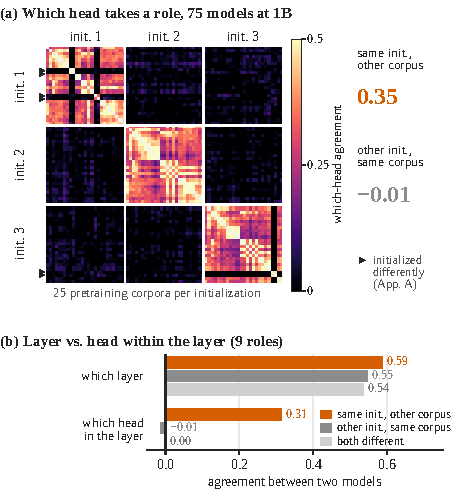
\includegraphics[width=\columnwidth]{figures/fig1_hook.pdf}
  \caption{\textbf{Models that share an initialization agree on which heads take each role.}
  (a)~Agreement on \emph{which} head in a layer takes a role (within-layer rank correlation of head scores, mean over induction, previous-token and retrieval maps) between all 75 one-billion-parameter DataDecide models, three initializations $\times$ 25 corpora, ordered by initialization.
  Bright blocks: models that share an initialization agree on every corpus; models that share only a corpus do not.
  $\blacktriangleright$: six runs initialized differently from their label (\S\ref{sec:trace}), excluded from all means.
  (b)~The two levels of a role map, mean over nine roles: the layer profile is similar for all pairs, the head within the layer only for pairs that share an initialization.}
  \label{fig:hook}
\end{figure}

Mechanistic interpretability describes a model through the roles of its components: an induction head completes a pattern seen earlier in the context \citep{olsson2022context}, a previous-token head attends to the preceding position, and retrieval heads copy a fact from the context into the prediction \citep{wu2025retrieval}.
When a model is trained again, its algorithms tend to recur while the components that implement them change \citep{chughtai2023toy,gurnee2024universal,tigges2024llm,bali2026quantifying}.
Two sources of this change are confounded.
Studies of seed variability retrain on a fixed corpus \citep{sellam2022multiberts,vanderwal2025polypythias,bali2026quantifying}, and studies that relate mechanisms to data vary the data under one initialization or many unrelated ones \citep{chan2022data,singh2024needs,chen2026mechanistic}.
Neither design can tell whether the head that takes a role is chosen by the initialization, by the data, or by neither.

We separate the two with a natural experiment that public pretraining suites already contain.
DataDecide \citep{magnusson2025datadecide} trains three initializations on up to 25 corpora at each of 14 sizes, and Pythia \citep{biderman2023pythia} trains one initialization on the Pile and on the deduplicated Pile at every size up to 12B parameters.
Comparing models that share an initialization but not a corpus with models that share a corpus but not an initialization shows how much each factor contributes.
For nine head roles we ask two questions: which layer hosts the role, and which head within that layer takes it.
Heads within a layer are interchangeable, so independently initialized models agree on the second question only by chance, which gives every comparison a baseline of zero (\S\ref{sec:setup}).

The two questions have different answers (Figure~\ref{fig:hook}).
All models largely agree on the layer.
Only models that share an initialization agree on the head within the layer, and they do so across corpora: under one initialization, the same head of layer~7 is the strongest induction head on 14 of 25 corpora (chance: 1.6).
The agreement holds for all nine roles, at all 14 DataDecide sizes and in Pythia up to 12B, and it is specific enough to tell which initialization a model came from.
Comparing layouts without labels, we found six DataDecide checkpoints that, as their released weights confirm, were initialized differently from their label (\S\ref{sec:trace}).

We then ask when the assignment is made and what decides how much of it carries over to another corpus.
In controlled pretraining, switching the corpus or perturbing the weights during the first 1\% of training reassigns the roles; a few percent later, a model returns to its assignment even after noise as large as its weights, and a switch of corpus rewrites only part of it, less the later it comes (\S\ref{sec:when}).
How much of the assignment two corpora share follows the similarity of their content words, and how strongly the initialization decides it at all follows the learning rate per batch token, which also explains why larger DataDecide models agree more (\S\ref{sec:conditions}).

Finally, we ask whether the initialization's effect on heads carries over to behaviour (\S\ref{sec:boundary}).
How strong a circuit becomes, when it forms and how a model scores on 10 benchmarks follow the corpus, and no initialization does consistently better across corpora.
A case study on one data component makes the division concrete.
Removing Flan, 1--2\% of Dolma~1.7, changes how models use a counterfactual context introduced by Flan's template \tmpl{Question:}, while the head layout of these models stays as close to its seed-matched siblings as under any other change of corpus.
The attention that Flan adds to the context after \tmpl{Question:} is spread over the heads that already attend to it: the data changes what the existing retrieval heads do, not which heads they are.

Our contributions are:
\begin{itemize}[leftmargin=*,itemsep=1pt,topsep=2pt]
  \item A seed $\times$ corpus design built from public suites at 21 sizes from 4M to 12B parameters, with a measurement that separates which layer from which head hosts a role and a permutation-symmetry baseline (\S\ref{sec:setup}).
  \item Evidence that which head within a layer takes each role follows the shared initialization rather than the corpus, at every size and for every role we measure, together with an audit of the suites' initializations (\S\ref{sec:trace}).
  \item Controlled experiments that locate when the assignment is fixed and identify corpus content and the stochastic-gradient noise scale as what determines how much of it is kept (\S\ref{sec:when}, \S\ref{sec:conditions}).
  \item Evidence that this structural effect does not carry over to behaviour, with a case study of a template habit that 1--2\% of the pretraining data strengthens while the head layout is preserved, and its consequences for knowledge-conflict evaluation (\S\ref{sec:boundary}).
\end{itemize}

\section{Setup and Measurement}
\label{sec:setup}

\paragraph{Initializations crossed with corpora.}
DataDecide pretrains OLMo-style models at 14 sizes (4M--1B parameters) on 25 corpus recipes---C4, DCLM and its quality-filtered variants, Dolma~1.6/1.7 and their ablations, Falcon RefinedWeb variants, FineWeb-Edu/-Pro and mixtures---each with three seeds.
Within a size, a seed's initial weights are shared across recipes, so each initialization has been trained on up to 25 corpora.
Pythia trains a standard and a deduplicated model from identical initial weights at every size; we use 70M--12B, with the independently initialized PolyPythias \citep{vanderwal2025polypythias} as a reference.
A DataDecide seed sets both the initial weights, which we check for every run (Appendix~\ref{app:audit}), and the data order. The order is not tied to any head and yields different batches on different corpora, so of what seed-matched runs share, only the initial weights can favour a particular head.
Model pairs fall into three types: \emph{same initialization, other corpus} (seed-matched pairs); \emph{other initialization, same corpus}; and both different.

\paragraph{Head-role maps.}
For each model we compute a [layer $\times$ head] map for each of nine roles from fixed probe material (Appendix~\ref{app:roles}): induction, previous-token, retrieval (attention from the answer position to the context entity in knowledge-conflict prompts), attention sink \citep{xiao2024efficient}, duplicate-token, current-token, two-back and delimiter heads, and each head's OV copying score, which is computed from the weights alone \citep{elhage2021mathematical}.

\paragraph{Two levels of agreement.}
A role map says which \emph{layer} hosts a role and which \emph{head} within the layer takes it.
We compare two models on the first with the rank correlation of their per-layer profiles and on the second with the \emph{which-head agreement}: the Spearman correlation of head scores within each layer, averaged over layers.

\paragraph{The chance baseline.}
Permuting the heads of a layer, together with their query, key, value and output weights, leaves the network's function unchanged; the initialization distribution and gradient-based training respect this symmetry.
Two independently initialized models therefore agree on which head takes a role only by chance, and their expected which-head agreement is exactly zero, whatever their corpora (Lemma~\ref{lem:symmetry}, Appendix~\ref{app:lemma}).
Agreement above zero between models trained on different corpora thus measures what their shared initialization carries through training.

\paragraph{Behaviour.}
We use DataDecide's 11 benchmark evaluations, circuit strength and developmental timing, and \emph{context trust}: on knowledge-conflict prompts that state a counterfactual fact, the log-probability margin of the counterfactual over the memorized answer, on facts the model knows \citep{li2025taming,du2024context}.

\section{Heads Follow the Initialization}
\label{sec:trace}

\begin{figure*}[t]
  \centering
  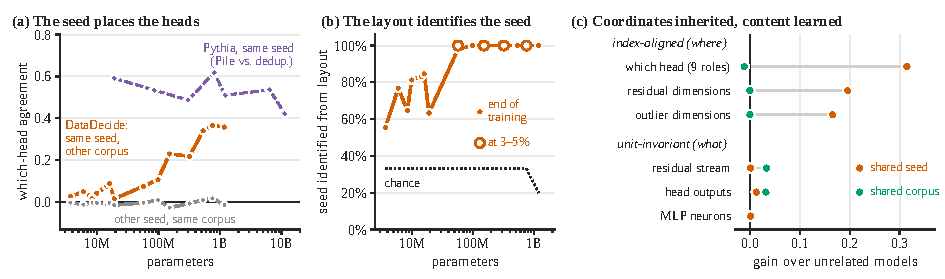
\includegraphics[width=\textwidth]{figures/fig2_innate.pdf}
  \caption{\textbf{The trace across sizes, as an identifier, and in other quantities.}
  (a)~Which-head agreement (mean over induction, previous-token and retrieval maps) for DataDecide pairs with the same initialization and different corpora and with different initializations and the same corpus, at 14 sizes, and for Pythia's two models from one initialization, up to 12B.
  (b)~Identifying a model's initialization from its head layout, leaving its corpus out, at the end of training and at 3--5\% of training.
  (c)~Similarity gained over unrelated models by sharing the initialization or the corpus: the initialization is shared in index-aligned quantities, the corpus in unit-invariant ones.}
  \label{fig:trace}
\end{figure*}

% generated by scripts/tables_acl.py -- do not edit by hand
\begin{table}[t]
  \centering
  \footnotesize
  \setlength{\tabcolsep}{3.3pt}
  \begin{tabular}{@{}lccc@{}}
    \multicolumn{4}{@{}l}{\textit{(a) DataDecide 1B, 3 seeds $\times$ 25 corpora (69 models)}} \\
    \toprule
    Role & same init. & other init. & gap, 95\% CI \\
    \midrule
    Two-back & 0.43 & 0.00 & [0.40, 0.46] \\
    Previous-token & 0.42 & $-$0.01 & [0.40, 0.47] \\
    Duplicate-token & 0.36 & $-$0.02 & [0.36, 0.41] \\
    Induction & 0.33 & $-$0.02 & [0.32, 0.37] \\
    Current-token & 0.32 & $-$0.02 & [0.31, 0.36] \\
    Retrieval & 0.31 & 0.00 & [0.28, 0.35] \\
    Delimiter & 0.22 & $-$0.01 & [0.20, 0.25] \\
    Attention sink & 0.18 & $-$0.01 & [0.16, 0.23] \\
    OV copying (weights) & 0.25 & $-$0.01 & [0.25, 0.29] \\
    \bottomrule
  \end{tabular}

  \vspace{6pt}
  \begin{tabular}{@{}lcccc@{}}
    \multicolumn{5}{@{}l}{\textit{(b) Pythia, one initialization: Pile vs.\ deduplicated Pile}} \\
    \toprule
    Size & induction & prev.-token & retrieval & null \\
    \midrule
    70M & -- & 0.60 & 0.58 & 0.26 \\
    160M & 0.49 & 0.58 & 0.53 & 0.14 \\
    410M & 0.47 & 0.55 & 0.45 & 0.09 \\
    1B & 0.56 & 0.72 & 0.58 & 0.16 \\
    1.4B & 0.48 & 0.54 & 0.50 & 0.09 \\
    6.9B & 0.53 & 0.60 & 0.49 & 0.06 \\
    12B & 0.38 & 0.51 & 0.38 & 0.04 \\
    12B, at 2.1\% & 0.55 & 0.60 & 0.45 & 0.04 \\
    \bottomrule
  \end{tabular}
  \caption{\textbf{Models with the same initialization agree on which head takes each role.} Which-head agreement
  (within-layer Spearman of head scores). (a)~All nine roles at 1B for models with the same initialization trained on
  different corpora and with different initializations trained on the same corpus; the gap's interval is a recipe
  bootstrap. (b)~Pythia's two models from one initialization; null:
  95th percentile after permuting heads within layers; no induction head at 70M.}
  \label{tab:roles}
\end{table}


\paragraph{Same initialization, same heads.}
In the 1B crossing, models with the same initialization agree on which head within a layer takes each role, while models with different initializations agree at chance, even on the same corpus (Table~\ref{tab:roles}a, Figure~\ref{fig:hook}).
This holds for all nine roles (0.18--0.43 against $-0.02$ to $0.00$), including the copying score computed from the weights alone, with five initializations at 1B, and on corpus pairs that share no data source.
Agreement is not limited to the ranking of weak heads: in the three layers where a role is strongest, the strongest head of two seed-matched models is the same one 2--5 times as often as chance (12--30\% against 6\%; Appendix~\ref{app:roles}).
When every head's within-layer rank is decomposed into initialization, corpus and residual components, the initialization is significant for 66--79\% of heads, that is, an initialization favours the same heads across corpora; the corpus main effect, which the symmetry rules out, is at the false-positive rate (4--7\%).
The agreement holds at all 14 DataDecide sizes and grows with size (Figure~\ref{fig:trace}a; Spearman with log parameters 0.81--0.92).
In Pythia, the two models from one initialization agree at every size from 70M to 12B, far above a permutation null (Table~\ref{tab:roles}b), while independently initialized PolyPythias agree at chance.

\paragraph{Depth is shared across models.}
The layer profile of each role agrees at 0.4--0.7 for every pair type (Figure~\ref{fig:hook}b), and all 75 1B models implement in-context copying with the same two-step algorithm, a previous-token head composing with an induction head.
Where in depth a role lives and how it is computed are largely common to all models; the initialization, not the corpus, biases which of the interchangeable heads in a layer carries it.

\paragraph{The layout is specific to the initialization.}
We hold out a model, compare its head layout with the models trained from each initialization on the \emph{other} corpora, and assign it to the closest one.
From 60M parameters on, this identifies the initialization with 98--100\% accuracy (chance: 33\%, or 20\% with five seeds), including all 69 verified 1B models, and already at 3--5\% of training (Figure~\ref{fig:trace}b, Table~\ref{tab:sizes}); in Pythia, the true sibling ranks first among ten candidates at all three sizes with independently initialized alternatives.
Applied without labels to the 75 1B models, the layout singles out six runs that agree with none of their nominal siblings but pairwise with each other (Figure~\ref{fig:hook}a, $\blacktriangleright$).
Their released weights confirm that these runs were not initialized from their seed's weights (correlation 0.000) and that each pair shares an initialization of its own (Table~\ref{tab:audit}).

\paragraph{What carries the trace.}
Seed-matched models on different corpora have drifted far apart: their weights correlate at only 0.01--0.04 (other pairs 0.000), enough to identify the initialization (Table~\ref{tab:ident}), they are not linearly connected (loss barrier 7.5 nats, against 7.8 for unrelated models; \citealp{frankle2020linear}), and under unit-invariant measures, CKA \citep{kornblith2019similarity} and best-match similarity, their representations are no closer than those of unrelated models (Figure~\ref{fig:trace}c).
What they share are index-aligned quantities: which head hosts a role, and which residual dimensions carry most variance (0.20 vs.\ 0.00) and the massive outlier activations (0.17 vs.\ 0.00).
The head layout is the functional form of this trace.

\section{When the Assignment Is Fixed}
\label{sec:when}

\begin{figure}[t]
  \centering
  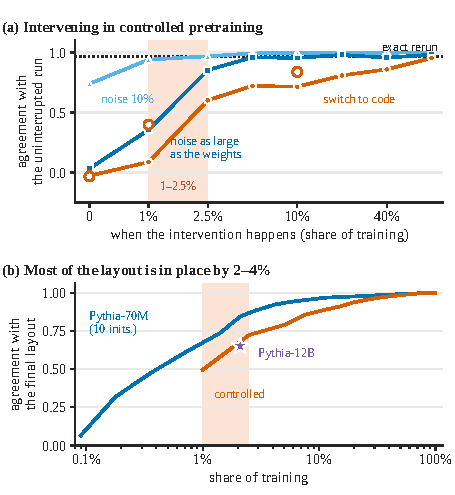
\includegraphics[width=\columnwidth]{figures/fig3_critical.pdf}
  \caption{\textbf{The assignment is fixed early.}
  (a)~Controlled pretraining (4 layers $\times$ 8 heads, 10k steps): agreement of the final layout with the uninterrupted run after switching the corpus to code or adding Gaussian noise to every weight at a given step; hollow circles: a 12-layer model.
  (b)~Agreement of the layout with its own final layout during training, in public suites and controlled runs; star: Pythia-12B at 2.1\%.
  Shaded: 1--2.5\% of training.}
  \label{fig:when}
\end{figure}

% generated by scripts/tables_acl.py -- do not edit by hand
\begin{table}[h]
  \centering
  \footnotesize
  \setlength{\tabcolsep}{3pt}
  \begin{tabular}{@{}rrcccc@{}}
    \toprule
    Step & Share & \makecell{Switch\\to code} & \makecell{Noise\\100\%} & \makecell{Noise\\10\%} & \makecell{Code, 12\\layers} \\
    \midrule
    0 & 0\% & $-$0.03 & 0.03 & 0.74 & $-$0.03 \\
    100 & 1\% & 0.09 & 0.36 & 0.94 & 0.40 \\
    250 & 2.5\% & 0.60 & 0.85 & 0.97 & -- \\
    500 & 5\% & 0.72 & 0.96 & 0.99 & -- \\
    1000 & 10\% & 0.71 & 0.95 & 0.99 & 0.84 \\
    2000 & 20\% & 0.81 & 0.98 & 1.00 & -- \\
    4000 & 40\% & 0.86 & 0.96 & 1.00 & -- \\
    8000 & 80\% & 0.95 & 0.98 & 1.00 & -- \\
    \midrule
    \multicolumn{2}{@{}l}{exact rerun} & \multicolumn{4}{c}{0.97} \\
    \bottomrule
  \end{tabular}
  \caption{\textbf{The critical period in numbers.} Which-head agreement (mean of induction and previous-token maps)
  between the final layout of a run intervened on at a given step and the untouched run. Step 0 for the code switch:
  the same seed trained on code from scratch.}
  \label{tab:critical}
\end{table}


\paragraph{Intervening during training.}
We pretrain small Llama-style models on C4 and branch them at step $k$ of 10{,}000, either switching the corpus to source code or adding Gaussian noise to every weight (Figure~\ref{fig:when}a, Table~\ref{tab:critical}).
Up to $k = 100$ (1\% of training), both interventions reassign the roles: after a switch to code, agreement with the uninterrupted run is 0.09, and noise as large as the weights leaves 0.03 at step 0 and 0.36 at step 100.
From $k = 250$ (2.5\%) on, the model returns to its assignment after the same noise (0.85 at 2.5\%, 0.95--0.98 from 5\%, the level of an exact rerun).
A switch to code still rewrites part of the layout, a smaller part the later it comes: agreement is 0.60 at 2.5\%, 0.71 at 10\% and 0.95 at 80\%.
A 12-layer model behaves alike: a switch to code at 1\% keeps 0.40 of the layout and at 10\% 0.84, while training on code from the start keeps none.

\paragraph{What closes the window.}
The early steps are also the warm-up of the learning rate (300 steps), and the branches inherit the optimizer's state, so we repeat the noise branches with a 1{,}000-step warm-up and, separately, with a freshly initialized optimizer (Appendix~\ref{app:warmup}).
With the longer warm-up the window closes later in steps (0.70 at 2.5\%, 0.87 from 5\%), and the two schedules align when agreement is plotted against the learning applied before the intervention, the cumulative learning rate (Figure~\ref{fig:warmup}).
Resetting the optimizer changes little (0.81, 0.91 and 0.97 at 2.5, 5 and 10\%).
The window thus tracks the amount of early learning more closely than the number of steps, and the assignment it leaves is held in the parameters rather than in the optimizer state.

\paragraph{Public suites.}
The public models also settle early (Figure~\ref{fig:when}b).
The same-initialization agreement of the DataDecide 1B models reaches its final level by 3.6\% of training, Pythia's previous-token heads stabilize by about 2\%, and Pythia-12B's two models already share their layout at 2.1\% (Table~\ref{tab:roles}b).
Before training, none of the statistics of a head's initial weights or initial gradient that we tested predicts which head will take a role, so the assignment is not readable at step 0; it is set by the first steps of training on top of the initialization.

\section{What Decides How Much Is Kept}
\label{sec:conditions}

\begin{figure}[t]
  \centering
  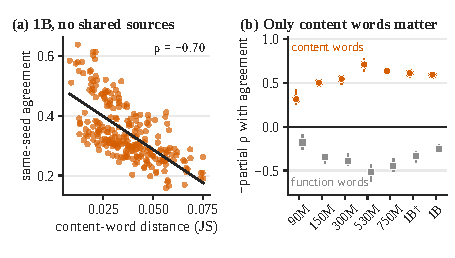
\includegraphics[width=\columnwidth]{figures/fig5_content.pdf}
  \caption{\textbf{Similar content words, similar heads.}
  (a)~1B pairs of DataDecide corpora that share no data source: Jensen--Shannon distance between their content-word distributions vs.\ the which-head agreement of same-initialization models trained on them.
  (b)~Negative partial Spearman correlation between distance and agreement for content words (controlling for function words) and for function words (controlling for content words), by size; bars span the three roles; $\dagger$: 1B with five seeds at 10\% of training.}
  \label{fig:content}
\end{figure}

The agreement between same-initialization models varies: across corpus pairs, across sizes and across training setups.
Two quantities track this variation.

\paragraph{Corpus similarity.}
Across DataDecide's corpus pairs, the Jensen--Shannon distance between two corpora's unigram distributions predicts how closely an initialization's layout recurs on both.
The relation holds at every size from 60M on and strengthens with size (Spearman $-0.20$ to $-0.33$ at 60M, $-0.65$ to $-0.83$ from 300M on, $-0.76$ to $-0.80$ across the 300 corpus pairs at 1B; Mantel $p < 0.001$ from 90M; Table~\ref{tab:sizes}), on pairs that share no data source ($-0.36$ to $-0.82$), and after partialling out source overlap.
Bigram distance predicts less ($-0.55$ to $-0.62$ at 1B).
Splitting the vocabulary into function words \citep{yang2026function} and content words shows which part of the distribution matters (Figure~\ref{fig:content}).
Content-word distance predicts agreement at every size ($\rho$ from $-0.23$ to $-0.69$), also when function-word distance is controlled (partial $\rho$ $-0.25$ to $-0.78$), whereas function-word distance, once content words are controlled, no longer predicts lower agreement (its partial $\rho$ turns positive, $\ge 0.09$, as two collinear distances do); the English web corpora in DataDecide use function words alike.
Controlled pretraining extends the relation to more distant corpora: C4 and scientific papers share the layout (0.19 $\pm$ 0.06 over nine initializations), pairs involving source code share none ($\approx$ 0), and Pythia's two versions of the Pile, nearly identical in content, share it most.

\paragraph{Gradient noise.}
Which head takes a role is settled when the symmetry between heads breaks early in training, by the initialization together with the gradient noise of those steps.
The noise of stochastic gradients scales with the learning rate per example in a batch \citep{smith2018bayesian,jastrzebski2018three}, and lowering it lets the initialization decide more.
At fixed model size, runs that differ only in the order of their batches agree 0.43 with 16-sequence batches and 0.90 with 512-sequence batches, and same-initialization agreement between C4 and scientific papers rises from 0.01 to 0.22 (Appendix~\ref{app:temperature}); tripling the learning rate acts like quartering the batch.
This can account for the growth with size in DataDecide: its recipes lower the learning rate per batch token 140-fold from 4M to 1B, whereas a 30$\times$ larger controlled model at a fixed rate keeps no more of its initialization, and Pythia, trained with large batches at every size, keeps it at 70M.

\section{Behaviour Follows the Corpus}
\label{sec:boundary}

\begin{table}[t]
  \centering
  \footnotesize
  \setlength{\tabcolsep}{2.4pt}
  \begin{tabular}{@{}llr@{}}
    \toprule
    Property & Follows & Key statistic \\
    \midrule
    Which head takes a role & \byinit{initialization} & 0.18--0.43 vs.\ 0.00 \\
    Residual coordinates & \byinit{initialization} & 0.20 vs.\ 0.00 \\
    Layer that hosts a role & all models & 0.4--0.7, all pairs \\
    Copying algorithm & all models & 75 / 75 models \\
    Circuit strength & \bycorpus{corpus} & 4 / 6 measures \\
    Onset of induction heads & \bycorpus{corpus} & 81\% vs.\ 0\% \\
    Representations & \bycorpus{corpus} & CKA, best match \\
    10 benchmarks, 14 sizes & \bycorpus{corpus} & init.\ sig.\ 4--8\% \\
    Knowledge conflicts & \bycorpus{corpus} & init.\ sig.\ 0 / 12 \\
    \tmpl{Question:} habit & \bycorpus{corpus} & $+2.4$ nats \\
    \bottomrule
  \end{tabular}
  \caption{\textbf{Which properties follow the initialization and which the corpus.} Key statistic: same- vs.\ different-initialization agreement; variance share of corpus vs.\ initialization; or share of cells with a significant initialization effect (5\% is the false-positive rate).}
  \label{tab:map}
\end{table}

\paragraph{Strength, timing and performance follow the corpus.}
How strongly a circuit is expressed follows the corpus (significant corpus effect on 4 of 6 strength measures, initialization component $\approx$ 0), and so does when it forms: in controlled pretraining with six initializations and three corpora, the corpus explains 81\% of the variance in the onset of induction heads and the initialization none ($p$ = 0.0001 vs.\ 0.47).
Across 10 benchmarks and their average at 14 sizes, the initialization has a significant main effect in 3.9\% (accuracy) and 7.8\% (per-byte likelihood) of the 154 cells, about the 5\% expected by chance, and the corpus in 75\% and 98\% (median variance components: initialization 0.000, corpus 0.49--0.83; Table~\ref{tab:benchmarks}); behaviour under knowledge conflict shows no initialization effect in any of 12 conditions.
What the initialization does contribute is specific to the corpus it is trained on (with one run per cell, interaction and run-to-run noise are not separable): an initialization that does well on one corpus is no more likely to do well on another (Table~\ref{tab:map}).

\subsection{Case Study: A Data Component and the \tmpl{Question:} Template}
\label{sec:question}

\begin{figure}[t]
  \centering
  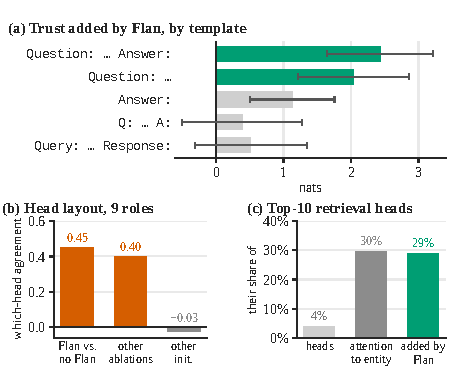
\includegraphics[width=\columnwidth]{figures/fig4_flan.pdf}
  \caption{\textbf{Flan changes behaviour, not the head layout} (1B).
  (a)~Flan minus no-Flan models: added trust in a counterfactual context relative to a declarative prompt, by template ($\pm$ SE over initializations).
  (b)~Which-head agreement (mean over nine roles) of same-initialization pairs with and without Flan, of same-initialization pairs of other Dolma~1.7 ablations, and of different-initialization pairs.
  (c)~The ten strongest retrieval heads of each Flan model: their share of all heads, of the attention to the context entity, and of the attention that Flan adds after \tmpl{Question:} (relative to \tmpl{Q:}).}
  \label{fig:flan}
\end{figure}

% generated by scripts/tables_acl.py -- do not edit by hand
\begin{table}[t]
  \centering
  \footnotesize
  \setlength{\tabcolsep}{3.5pt}
  \begin{tabular}{@{}lrrr@{}}
    \toprule
    Ending after the context & \makecell[r]{count in\\Dolma 1.7} & \makecell[r]{Flan\\effect} & SE \\
    \midrule
    \tmpl{Question:} $q$ \tmpl{Answer:} & 11.3M / 9.6M & +2.43 & 0.79 \\
    \tmpl{Question:} $q$ & 11.3M & +2.04 & 0.83 \\
    \tmpl{Answer:} & 9.6M & +1.13 & 0.63 \\
    \tmpl{Q:} $q$ \tmpl{A:} & 38.4M / 6.9M & +0.39 & 0.89 \\
    \tmpl{Query:} $q$ \tmpl{Response:} & 0.15M / 0.75M & +0.52 & 0.83 \\
    \tmpl{Question:} $q'$ \tmpl{Answer:} & as first row & +3.06 & 1.42 \\
    \midrule
    declarative (no question) & -- & +0.20 & 0.50 \\
    \bottomrule
  \end{tabular}
  \caption{\textbf{The habit is keyed to Flan's literal template.} Flan minus no-Flan models (1B, three initializations each):
  added trust in the counterfactual context relative to a declarative ending, in nats. Example:
  \textit{The capital of France is Rome.} \tmpl{Question:} \textit{What is the capital of France?} \tmpl{Answer:}
  \textit{The capital of France is}~\dots; $q'$ asks about another entity. Marker counts: occurrences in the
  pretraining corpus. The last row is the raw trust difference for the declarative ending.}
  \label{tab:template}
\end{table}


The previous results concern where roles are placed and show that performance does not follow the placement.
This case study asks the converse question for one data component that clearly changes behaviour: does it move the head layout, and where is the behaviour it teaches expressed?
We compare seed-matched models trained with and without the component.
Dolma~1.7 contains about 1--2\% of Flan instruction data \citep{longpre2023flan,soldaini2024dolma}, and DataDecide trains a Dolma~1.7 recipe with Flan removed from the same initializations.
We compare the two on knowledge-conflict prompts from ParaConflict \citep{li2025taming}: one sentence asserts a counterfactual fact (``The capital of France is Rome.'') and is followed by a declarative continuation or by a question in Flan's format (\tmpl{Question: What is the capital of France? Answer:}).

\paragraph{Flan adds trust after \tmpl{Question:}.}
Removing Flan lowers the 1B models' trust in the counterfactual context by 1.3--3.5 nats across four kinds of context when the prompt is a question, and leaves declarative prompts and the models' knowledge of the facts unchanged.
The share of questions on which a model ignores a one-sentence context and answers from memory rises from 1.9\% to 14.3\%.
The effect is tied to Flan's own wording (Figure~\ref{fig:flan}a, Table~\ref{tab:template}): at 1B \tmpl{Question:} alone carries most of it, and across the seven sizes Flan's template exceeds the equivalent \tmpl{Q:}~\dots~\tmpl{A:} by $0.93 \pm 0.29$ nats and \tmpl{Query:}~\dots~\tmpl{Response:} by $0.98 \pm 0.32$, although \tmpl{Q:} is three times as frequent as \tmpl{Question:} in Dolma~1.7; a question about a different entity triggers it as strongly.
It is present from 3.6\% of pretraining, at sizes from 60M on, on PopQA counterfactuals \citep{mallen2023popqa} and NQ-Swap \citep{longpre2021entity}, and in OLMo~2 \citep{olmo2024olmo2} after mid-training on a mixture with FLAN (Appendix~\ref{app:question}).

\paragraph{The layout is preserved.}
Seed-matched models with and without Flan agree on which head takes each role at 0.45 (mean over nine roles), as closely as seed-matched pairs of other Dolma~1.7 ablations (0.40), while different initializations agree at $-0.03$ (Figure~\ref{fig:flan}b).
Removing Flan changes the behaviour without lowering the agreement that the shared initialization produces.

\paragraph{Where the habit acts.}
To locate the habit, we measure each head's attention from the last prompt token to the counterfactual entity, the read-out of the retrieval role, and take the difference between \tmpl{Question:} and \tmpl{Q:} prompts.
Models trained with Flan attend more to the context after \tmpl{Question:} (summed over heads, $+0.54$), models without Flan less ($-0.21$).
The added attention is spread over the heads that already attend to the entity: the model's ten strongest retrieval heads carry 30\% of its attention to the entity and receive 29\% of the addition (30\% when the heads are chosen on held-out items; Figure~\ref{fig:flan}c), and models with the same initialization agree on where it falls (0.11, against $-0.03$ for different initializations).
Flan changes how much the existing retrieval heads attend after its template, not which heads retrieve.

\paragraph{Consequences for evaluation.}
Context-faithfulness and knowledge-conflict benchmarks commonly pose questions in exactly this format, and every public base model we tested trusts a counterfactual context more after \tmpl{Question:} than in a declarative prompt, by 1.0--4.6 nats, most of all the model pretrained with Flan (Table~\ref{tab:public}).
A score on such benchmarks therefore mixes faithfulness with a habit that a small slice of pretraining data strengthens and a change of template removes, which gives prompt-template sensitivity \citep{sclar2024quantifying,hua2025flaw,liu2026prompt} a concrete source in the pretraining corpus.

\section{Related Work}
\label{sec:related}

\paragraph{Seeds and training variability.}
Seed variation is a known source of irreproducibility in fine-tuning and pretraining \citep{reimers2017reporting,dodge2020fine,mccoy2020berts,sellam2022multiberts}, modelled as noise \citep{benitosantos2025robust} or studied as convergence across training \citep{fehlauer2025convergence,vanderwal2025polypythias}; SeedPrints \citep{tong2026seedprints} identifies a seed from output biases.
Crossing seeds with corpora separates the initialization from the data: its effect on head placement carries across corpora, its effect on behaviour does not.

\paragraph{Universality and stability of circuits.}
Hidden units of independently trained networks correspond only up to permutation \citep{li2016convergent,entezari2022role,ainsworth2023git}, and models fine-tuned from one pretrained checkpoint often stay in one basin \citep{neyshabur2020transferred}, though not always \citep{juneja2023linear}.
Algorithms recur across models while components vary \citep{chughtai2023toy,gurnee2024universal,tigges2024llm}; attention heads differ across retraining \citep{bali2026quantifying}, specialize along developmental trajectories \citep{wang2025differentiation}, and can be read from their parameters \citep{elhelo2025maps}.
Without any alignment, a shared initialization makes heads correspond across corpora, although the models are not linearly connected.

\paragraph{Data and the formation of mechanisms.}
Data properties decide whether in-context learning emerges \citep{chan2022data,singh2024needs}, and individual training examples shape when a head forms \citep{chen2026mechanistic}.
We find that the corpus sets whether, when and how strongly a mechanism forms, while the initialization sets where.
Early training is known to be decisive for what a network can still learn \citep{achille2019critical} and for which basin it ends in \citep{frankle2020linear}; we show the same for which head takes which role.

\paragraph{Knowledge conflicts and prompt format.}
Whether a model follows a counterfactual context or its memory depends on the context's form and the model's confidence \citep{longpre2021entity,xie2024adaptive,du2024context}, is mediated by competing mechanisms \citep{ortu2024competition}, and shifts with the prompt's wording \citep{zhou2023context,sclar2024quantifying,hua2025flaw,liu2026prompt}; synthetic pretraining shows which data properties make models use both sources \citep{kim2026training}.
We trace one such format effect to a 1--2\% slice of natural pretraining data.

\section{Discussion and Conclusion}
\label{sec:conclusion}

\paragraph{Interpretability.}
A circuit found in one model generalizes to other models in its algorithm and its layers; its head labels transfer only partly, and only to models with the same initialization.
Ablating the ten heads that matter most for induction in a same-initialization sibling trained on another corpus does 19.5\% of the damage of ablating the model's own, against 10\% for random heads in the same layers and 2.0\% for heads found in a different-initialization model trained on the \emph{same} corpus (1B, six corpora).
Comparisons of circuits across training data should therefore match initializations, and seed-matched siblings in public suites provide such comparisons: their heads correspond, so differences between their circuits can be attributed to the data.

\paragraph{Training and evaluation.}
Larger batches or smaller learning rates make head assignments more reproducible across corpora; seed selection does not carry over between recipes.

\paragraph{Conclusion.}
Models trained from one initialization on different corpora agree on which heads take each role; the agreement is set by a small amount of early learning and grows with corpus similarity and lower gradient noise, while what the heads do follows the corpus.

\section*{Limitations}
We study decoder-only transformers with multi-head attention, pretrained on English corpora, up to 12B parameters, and define head roles through attention patterns and OV circuits; with grouped-query attention, heads are interchangeable only within and across groups, which changes the baseline.
Multilingual seed-crossed suites would test the corpus-similarity relation where function words differ across corpora, and other architectures can be added as such suites appear.
Our interventions during training use models of up to 12 layers; intervening on larger models in their first percent of training is the natural next step.
The template habit is one data component; why models key on \tmpl{Question:} rather than an equivalent marker, and which other instruction-data families install habits of their own, are open.
Which property of the initialization decides which head will take a role is likewise open.

\section*{Ethical Considerations}
We analyse publicly released models and datasets under their licences and train small models on public corpora; no human subjects are involved.
We report our audit of public checkpoints to support their correct use.

\bibliography{refs}

\appendix

\section{Auditing the Public Suites}
\label{app:audit}

% generated by scripts/tables_acl.py -- do not edit by hand
\begin{table}[h]
  \centering
  \scriptsize
  \setlength{\tabcolsep}{2.5pt}
  \begin{tabular}{@{}llccc@{}}
    \toprule
    DataDecide 1B recipe & seed & \makecell{step 0 vs.\\seed's step 0} & \makecell{step 2500 vs.\\seed's step 0} & \makecell{step 2500 vs.\\partner} \\
    \midrule
    DCLM QC 7\% FW2 & 1 & 0.00 & 0.00 & 0.11 \\
    DCLM QC 7\% FW3 & 1 & 0.00 & 0.00 & 0.11 \\
    Dolma 1.7 no math/code & 1 & 0.00 & 0.00 & 0.08 \\
    Dolma 1.7 no Reddit & 1 & 0.00 & 0.00 & 0.08 \\
    Falcon+CC QC orig.\ 10\% & 3 & 0.00 & 0.00 & 0.09 \\
    Falcon+CC QC Tulu 10\% & 3 & 0.00 & 0.00 & 0.09 \\
    \midrule
    \multicolumn{4}{@{}l}{genuine siblings (C4 vs.\ Dolma~1.7, same seed), step 2500} & 0.07--0.08 \\
    \bottomrule
  \end{tabular}
  \caption{\textbf{Six 1B runs were not initialized from their seed's weights.} Correlation of one attention weight
  matrix (block 5) between checkpoints. The other 69 runs share their seed's step-0 weights exactly.}
  \label{tab:audit}
\end{table}


\paragraph{Step-0 identity.}
Pythia's standard and deduplicated models have tensor-identical step-0 weights at 70M, 160M, 410M, 1.4B and 2.8B, rounding-level identical weights at 1B (correlation 0.99993) and identical files at 6.9B and 12B.
For DataDecide we compare one weight matrix of every released step-0 checkpoint with the step 0 of the same seed's C4 run, reading the tensor directly from the hosted files.

\paragraph{All sizes.}
Below 1B, we use for each size the recipes whose three seeds share their published step-0 weights (by file hash) and the checkpoint listed in Table~\ref{tab:sizes}: the final checkpoint up to 90M, and at larger sizes a checkpoint available for all selected runs (43--98\% of training; 11\% for the five-seed 1B set).
For every one of these 686 runs we compare the earliest training checkpoint (step 1{,}250; 2{,}500 at 1B) with the step-0 weights of every seed.
Each correlates with its own seed's step 0 (0.05--0.41, rising with size) and with no other seed's ($\le 0.009$), except one 1B run at 11\% of training (FineWeb-Pro, seed 3), which matches no seed and is excluded.

\paragraph{Training start.}
A published step-0 checkpoint need not be the state a run started from, so we compare the earliest training checkpoint with every candidate initialization.
The DataDecide 1B runs of C4, Dolma~1.7 and DCLM correlate at step 2{,}500 only with their own seed's step-0 weights (0.23 vs.\ 0.000).
PolyPythias' ``weight-seed'' variants at 160M, in contrast, were trained from the standard initialization: their step-1 weights equal the standard model's (correlation 1.0) and are unrelated to their own published step 0; we label them accordingly.

\paragraph{Six 1B runs with an unlisted initialization.}
Six 1B DataDecide runs disagree with all their nominal siblings in Figure~\ref{fig:hook}a: the DCLM-QC 7\% FineWeb-2/3 recipes and the Dolma~1.7 no-math-code / no-Reddit ablations of seed 1, and the Falcon-and-CC QC original / Tulu recipes of seed 3 (Table~\ref{tab:audit}).
Their published step-0 weights differ from their seed's, their step-2{,}500 weights correlate with no seed's step 0, and each pair's step-2{,}500 weights correlate with each other as strongly as those of two genuine siblings: each pair was trained from an initialization of its own.
All other 69 runs share their seed's step-0 weights exactly, so the layout flagged exactly the six runs that differ.
We exclude them from every same- and different-initialization comparison at 1B.

\paragraph{A near-duplicate Pythia pair.}
The released final checkpoint of pythia-2.8b-deduped is nearly identical to that of pythia-2.8b (attention-weight correlation 0.993, embedding correlation 0.985), whereas models trained from one initialization on different data retain a correlation of only 0.03--0.09 with it; we exclude the 2.8B pair.

\section{Head Roles}
\label{app:roles}
\textbf{Induction}: attention from the second copy of a random 128-token block to the token after its first occurrence (200 blocks).
\textbf{Previous-token}: attention to position $t-1$ on 50 natural texts (split-half reliability 0.99--1.00).
\textbf{Attention sink}: attention to position 0 on the same texts.
\textbf{Retrieval}: attention from the last prompt token to the counterfactual entity in the knowledge-conflict prompts.
\textbf{Duplicate-token}, \textbf{current-token}, \textbf{two-back} and \textbf{delimiter}: attention to an earlier copy of the current token, to itself, to $t-2$ and to punctuation, on natural text.
\textbf{OV copying}: the share of positive eigenvalue mass of the head's OV circuit composed with the embedding and unembedding \citep{elhage2021mathematical}, computed from weights alone.
An induction map is used only when the model has an induction head (maximum score $> 0.3$).
Split-half reliabilities are 0.99--1.00 for the previous-token, sink, current-token, two-back and delimiter maps, so differences in agreement between roles are not differences in measurement noise.

\paragraph{Agreement on the strongest head.}
Which-head agreement averages a rank correlation over all layers.
Restricted to the three layers where a role is strongest at 1B, it is as high or higher (0.19--0.47 for seed-matched pairs, $-0.07$ to $0.03$ for other pairs) than in the remaining layers (0.18--0.43).
In those three layers, the strongest head of two seed-matched models is the same in 12--30\% of cases across the nine roles (different initializations: 4--9\%; chance: 6\%), and their three strongest heads overlap by 27--48\% (chance: 19\%).
The example of Section~\ref{sec:intro} is the most consistent of the three initializations: under the other two, the most frequent strongest induction head wins on 11 of 21 and 9 of 23 corpora with an induction head.

\paragraph{Ablation-defined roles.}
Defining a head's role by the effect of ablating it rather than by its attention pattern gives the same picture, more weakly: maps of each head's contribution to induction and to context use agree at 0.10--0.12 between seed-matched 1B models trained on different corpora and at 0.00 between models with different initializations (six corpora, three initializations).

\section{Head Permutation Symmetry and the Chance Baseline}
\label{app:lemma}
\begin{lemma}
\label{lem:symmetry}
Let a layer have $H$ heads and let $\pi$ permute them together with their query, key, value and output blocks.
Assume (i) the initialization distribution is invariant under $\pi$; (ii) training is $\pi$-equivariant, i.e.\ the update applied to $\pi\theta$ is $\pi$ applied to the update of $\theta$ (true for gradient descent, Adam/AdamW, weight decay and global-norm clipping, as the loss is $\pi$-invariant); and (iii) the data and their order are independent of the initialization.
Let $w(\theta)$ be the head with the largest score for a role, computed from the network's internals, so that $w(\pi\theta) = \pi(w(\theta))$.
Then for every corpus $D$, $P(w(\theta_T) = h \mid D) = 1/H$, and two independently initialized models trained on any corpora $D, D'$ agree on the winning head with probability $1/H$; the expected within-layer rank correlation of their head scores is $0$.
\end{lemma}
\begin{proof}[Proof sketch]
By (i)--(ii), $\theta_T$ and $\pi\theta_T$ have the same distribution given $D$, so $w(\theta_T)$ is uniform over heads.
Independent initializations make $w$ and $w'$ independent, so they agree with probability $\sum_h (1/H)^2 = 1/H$; averaging over permutations sends any rank correlation to zero in expectation.
\end{proof}
The lemma fixes the baseline for pairs with independent initializations; it makes no prediction for pairs that share one, whose agreement is the quantity we measure.
Different-initialization pairs agree at $-0.02$ to $0.00$ for all nine roles (Table~\ref{tab:roles}a).

\section{Results at Every Size}
\label{app:sizes}
% generated by scripts/tables_acl.py -- do not edit by hand
\begin{table*}[t]
  \centering
  \footnotesize
  \setlength{\tabcolsep}{2.4pt}
  \begin{tabular}{@{}lrrrrrrrcr@{}}
    \toprule
    Parameters & \makecell[r]{Checkpoint\\(share)} & Recipes & Seeds & \makecell[r]{Same init.,\\other corpus} & \makecell[r]{Other init.,\\same corpus} &
    \makecell[r]{Init. ID\\(\%)} & \makecell[r]{Init. ID,\\early (\%)} & \makecell{$\rho$(corpus distance,\\agreement)} &
    \makecell[r]{LR per batch\\token ($10^{-9}$)} \\
    \midrule
    4M & 5{,}725 (100\%) & 18 & 3 & 0.03 & 0.00 & 56 & -- & -- & 213.6 \\
    6M & 9{,}182 (100\%) & 23 & 3 & 0.05 & $-$0.01 & 77 & -- & -- & 183.1 \\
    8M & 13{,}039 (100\%) & 17 & 3 & 0.02 & 0.00 & 65 & -- & -- & 167.8 \\
    10M & 15{,}117 (100\%) & 16 & 3 & 0.04 & 0.00 & 81 & 72 & -- & 152.6 \\
    14M & 21{,}953 (100\%) & 18 & 3 & 0.08 & $-$0.01 & 83 & -- & -- & 140.4 \\
    16M & 24{,}432 (100\%) & 13 & 3 & 0.09 & 0.00 & 85 & -- & -- & 135.8 \\
    20M & 14{,}584 (100\%) & 20 & 3 & 0.02 & $-$0.01 & 63 & 61 & -- & 64.1 \\
    60M & 29{,}042 (100\%) & 17 & 3 & 0.08 & 0.00 & 98 & 100 & $-$0.20 to $-$0.33 & 29.5 \\
    90M & 29{,}901 (100\%) & 20 & 3 & 0.11 & 0.01 & 100 & -- & $-$0.43 to $-$0.50 & 15.0 \\
    150M & 37{,}500 (98\%) & 15 & 3 & 0.23 & $-$0.03 & 100 & 100 & $-$0.47 to $-$0.64 & 10.7 \\
    300M & 45{,}000 (98\%) & 15 & 3 & 0.22 & $-$0.01 & 100 & 100 & $-$0.69 to $-$0.78 & 5.0 \\
    530M & 51{,}250 (89\%) & 10 & 3 & 0.34 & 0.01 & 100 & -- & $-$0.65 to $-$0.71 & 3.1 \\
    750M & 27{,}500 (43\%) & 10 & 3 & 0.37 & 0.02 & 100 & 100 & $-$0.66 to $-$0.77 & 2.1 \\
    1B$^\dagger$ & 7{,}500 (11\%) & 10 & 5 & 0.36 & $-$0.01 & 100 & -- & $-$0.75 to $-$0.83 & 1.5 \\
    1B & 69{,}369 (100\%) & 25 & 3 & 0.35 & $-$0.01 & 100 & -- & $-$0.76 to $-$0.80 & 1.5 \\
    \bottomrule
  \end{tabular}
  \caption{\textbf{DataDecide at every size.} The checkpoint used (DataDecide revision \texttt{step<N>-seed-<seed>}; share
  of the default seed's training), the recipes whose three seeds share their step-0 weights, which-head agreement (mean
  over induction, previous-token and retrieval maps; induction only where models have induction heads), leave-one-corpus-out
  identification of the initialization from the head layout at that checkpoint and at the earliest available one (3--9\% of training; chance 33\%, 20\% with five seeds), the Spearman correlation
  between unigram corpus distance and same-initialization agreement over corpus pairs (range over roles), and the recipe's
  learning rate per batch token. $\dagger$: five seeds at 11\% of training; last row: the verified three-seed crossing at
  the end of training. Every run starts from its labelled initialization (Appendix~\ref{app:audit}).}
  \label{tab:sizes}
\end{table*}

Table~\ref{tab:sizes} lists, for every DataDecide size, the recipes and seeds used, same- and different-initialization agreement, initialization identification at the end of training and in the earliest checkpoints, the corpus-distance relation and the recipe's learning rate per batch token.
Agreement is weak up to 20M parameters, where most models have not yet formed an induction head, and strong from 150M on.

\section{Identifying the Initialization}
\label{app:ident}
% generated by scripts/tables_acl.py -- do not edit by hand
\begin{table*}[t]
  \centering
  \footnotesize
  \setlength{\tabcolsep}{6pt}
  \begin{tabular}{@{}lrrrrrr@{}}
    \toprule
    & \multicolumn{3}{c}{Identified (\%)} & \makecell[r]{Weight\\correlation} & \multicolumn{2}{c}{SeedPrints $z$} \\
    \cmidrule(lr){2-4} \cmidrule(l){6-7}
    Size & head layout & weights & SeedPrints & same init. & same init. & same corpus \\
    \midrule
    4M & 56 & 98 & 94 & 0.022 & 9.5 & 1.0 \\
    6M & 77 & 100 & 91 & 0.016 & 8.7 & 0.7 \\
    8M & 65 & 100 & 94 & 0.013 & 8.7 & 1.6 \\
    10M & 81 & 100 & 88 & 0.011 & 8.4 & 1.5 \\
    14M & 83 & 100 & 94 & 0.009 & 7.8 & 3.6 \\
    16M & 85 & 100 & 82 & 0.009 & 7.1 & 3.4 \\
    20M & 63 & 100 & 97 & 0.016 & 8.1 & 2.3 \\
    60M & 98 & 100 & 100 & 0.010 & 11.9 & 5.1 \\
    90M & 100 & 100 & 100 & 0.012 & 13.3 & 3.9 \\
    150M & 100 & 100 & 100 & 0.013 & 24.0 & 5.1 \\
    300M & 100 & 100 & 100 & 0.016 & 30.1 & 5.9 \\
    530M & 100 & 100 & 100 & 0.019 & 46.7 & 6.1 \\
    750M & 100 & 100 & 100 & 0.022 & 46.4 & 4.1 \\
    1B$^\dagger$ & 100 & 100 & 100 & 0.043 & 54.7 & 1.7 \\
    1B & 100 & 100 & 100 & 0.016 & 63.8 & 9.8 \\
    \bottomrule
  \end{tabular}
  \caption{\textbf{Identifying the initialization three ways.} Leave-one-corpus-out accuracy from the head layout,
  from the correlation of final weights (a fixed sample of 2M attention and MLP weights) and from SeedPrints
  \citep{tong2026seedprints}; mean weight correlation of same-initialization pairs, and mean SeedPrints statistic of
  same-initialization and of same-corpus, different-initialization pairs. $\dagger$: five seeds at 11\% of training.}
  \label{tab:ident}
\end{table*}

Table~\ref{tab:ident} compares identification from the head layout with two baselines on the same leave-one-corpus-out task.
Final weights identify the initialization at every size: same-initialization pairs keep a weight correlation of 0.01--0.04, other pairs 0.000.
SeedPrints \citep{tong2026seedprints}, a rank test on final hidden states for random token sequences, identifies it from 60M on; its statistic is also raised for pairs that share only a corpus, which the head layout and the weights are not.
On the six 1B runs with an unlisted initialization, all three methods agree: each run is closest to its partner run and to none of its nominal siblings.

\section{Controlled Pretraining}
\label{app:controlled}
Llama-style models (RMSNorm, SwiGLU, RoPE, untied embeddings, OLMo tokenizer): 4 layers $\times$ 8 heads, $d = 256$; and 12 layers $\times$ 12 heads, $d = 768$.
AdamW (learning rate $10^{-3}$, $\beta = (0.9, 0.95)$, weight decay 0.1), 300 warm-up steps, cosine decay to 10\%, batches of 64 $\times$ 512 tokens, 10{,}000 steps.
Corpora: the first 400M tokens of single DataDecide sources for web text (C4), code (StarCoder), scientific papers (peS2o) and books (Gutenberg).
Branches continue from the parent's saved model and optimizer state at step $k \in \{100, 250, 500, 1000, 2000, 4000, 8000\}$, either switching the corpus or adding $\epsilon \cdot \mathrm{std}(W) \cdot \mathcal{N}(0, 1)$ to every tensor (Table~\ref{tab:critical}).
At initialization the basin is finite: perturbations up to 1\% of the weight scale leave the layout unchanged (0.91--0.99), 10\% partly reassign it (0.74; 0.57 and 0.91 for the two initializations), and 100\% reassign it fully (0.03).

\section{Warm-up and Optimizer State}
\label{app:warmup}
\begin{figure}[h]
  \centering
  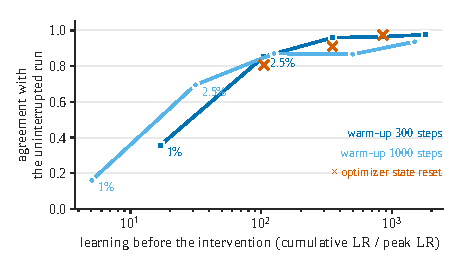
\includegraphics[width=\columnwidth]{figures/figA_warmup.pdf}
  \caption{\textbf{The window tracks cumulative learning.} Agreement of the final layout with the uninterrupted run after noise as large as the weights at 1, 2.5, 5, 10 and 20\% of training, against the cumulative learning rate before the intervention (in units of the peak rate), for warm-ups of 300 and 1{,}000 steps; crosses: branches with a freshly initialized optimizer (300-step warm-up). Means over two initializations and the induction and previous-token maps.}
  \label{fig:warmup}
\end{figure}
We repeat the noise branches of Appendix~\ref{app:controlled} with two parents whose learning rate warms up over 1{,}000 instead of 300 steps, branching at $k \in \{100, 250, 500, 1000, 2000\}$, and with branches that discard the parent's AdamW state at $k \in \{250, 500, 1000\}$.
A parent continued from its own step-2{,}000 state reproduces its final layout (0.995--1.00), so the comparisons are not limited by run-to-run noise.
With the longer warm-up, a switch to code keeps 0.41 of the layout at 2.5\% and 0.69 at 10\% (0.60 and 0.71 with the default warm-up).
Changing only the warm-up, with the same initialization and data order, changes part of the final layout (agreement 0.21--0.59 for induction and 0.62--0.67 for previous-token maps), another sign that the first steps of training help decide which head takes a role.

\section{Gradient Noise}
\label{app:temperature}
\begin{figure}[h]
  \centering
  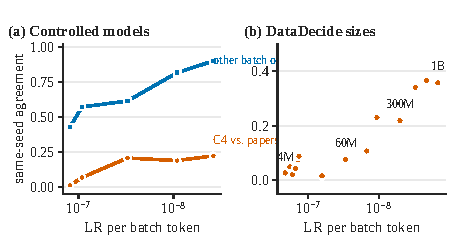
\includegraphics[width=\columnwidth]{figures/figA_temperature.pdf}
  \caption{\textbf{Less gradient noise, more agreement.} (a)~Controlled models at step 2{,}000: which-head agreement between runs that differ only in batch order, and between C4 and scientific-paper runs from one initialization, against the learning rate per batch token. (b)~DataDecide: same-initialization agreement against the recipe's learning rate per batch token.}
  \label{fig:temperature}
\end{figure}
% generated by scripts/tables_acl.py -- do not edit by hand
\begin{table}[h]
  \centering
  \footnotesize
  \setlength{\tabcolsep}{3.5pt}
  \begin{tabular}{@{}rrrcc@{}}
    \toprule
    Batch & LR & \makecell[r]{LR per batch\\token ($10^{-6}$)} & \makecell{other batch\\order} & \makecell{C4 vs.\\papers} \\
    \midrule
    16 & 1$\cdot 10^{-3}$ & 0.12 & 0.43 & 0.01 \\
    64 & 3$\cdot 10^{-3}$ & 0.09 & 0.57 & 0.07 \\
    64 & 1$\cdot 10^{-3}$ & 0.03 & 0.61 & 0.21 \\
    64 & 3$\cdot 10^{-4}$ & 0.01 & 0.82 & 0.19 \\
    512 & 1$\cdot 10^{-3}$ & 0.00 & 0.90 & 0.22 \\
    \bottomrule
  \end{tabular}
  \caption{\textbf{Gradient noise.} Same-initialization which-head agreement of previous-token maps at step 2{,}000 between runs
  that differ only in batch order, and between runs on C4 and on scientific papers.}
  \label{tab:temperature}
\end{table}

At fixed size we vary the batch (16, 64, 512 sequences) and the learning rate ($3\cdot10^{-3}$, $10^{-3}$, $3\cdot10^{-4}$) and read the layout at step 2{,}000, after the assignment is fixed (Table~\ref{tab:temperature}).
Order-only agreement is ordered by the learning rate per batch token, and tripling the learning rate acts like quartering the batch.

\section{Initialization Effects on Benchmarks}
\label{app:benchmarks}
% generated by scripts/tables_acl.py -- do not edit by hand
\begin{table*}[t]
  \centering
  \footnotesize
  \setlength{\tabcolsep}{4.5pt}
  \begin{tabular}{@{}lcccccccc@{}}
    \toprule
    & \multicolumn{4}{c}{Accuracy} & \multicolumn{4}{c}{Correct-answer likelihood per byte} \\
    \cmidrule(lr){2-5} \cmidrule(l){6-9}
    Benchmark & init. sig. & corpus sig. & init. share & corpus share & init. sig. & corpus sig. & init. share & corpus share \\
    \midrule
    ARC-Easy & 0/14 & 14/14 & 0.00 & 0.95 & 0/14 & 14/14 & 0.00 & 0.91 \\
    ARC-Challenge & 1/14 & 10/14 & 0.00 & 0.49 & 0/14 & 14/14 & 0.00 & 0.92 \\
    BoolQ & 0/14 & 7/14 & 0.00 & 0.25 & 2/14 & 13/14 & 0.00 & 0.55 \\
    CSQA & 0/14 & 12/14 & 0.00 & 0.55 & 1/14 & 14/14 & 0.01 & 0.56 \\
    HellaSwag & 2/14 & 13/14 & 0.00 & 0.60 & 2/14 & 14/14 & 0.00 & 0.96 \\
    MMLU & 1/14 & 13/14 & 0.00 & 0.87 & 1/14 & 14/14 & 0.00 & 0.95 \\
    OpenBookQA & 1/14 & 10/14 & 0.00 & 0.40 & 1/14 & 14/14 & 0.00 & 0.85 \\
    PIQA & 0/14 & 14/14 & 0.00 & 0.56 & 1/14 & 14/14 & 0.00 & 0.76 \\
    Social IQa & 0/14 & 10/14 & 0.00 & 0.30 & 2/14 & 13/14 & 0.00 & 0.48 \\
    WinoGrande & 1/14 & 3/14 & 0.00 & 0.07 & 1/14 & 13/14 & 0.00 & 0.79 \\
    OLMES average & 0/14 & 10/14 & 0.00 & 0.46 & 1/14 & 14/14 & 0.00 & 0.78 \\
    \bottomrule
  \end{tabular}
  \caption{\textbf{Initialization effects on benchmarks.} For each benchmark, the number of the 14 model sizes at which the initialization or the corpus
  has a significant main effect ($p < 0.05$, two-way ANOVA over recipes and seeds) and the median unbiased variance
  share of each factor across sizes.}
  \label{tab:benchmarks}
\end{table*}

Table~\ref{tab:benchmarks} breaks the benchmark analysis of \S\ref{sec:boundary} down by task.
The corpus is a significant factor on almost every task and size; the initialization reaches significance in 0--2 of 14 sizes per task, as expected by chance, and its median variance share is zero on every task.

\section{The Template Habit in Detail}
\label{app:question}
\begin{figure*}[t]
  \centering
  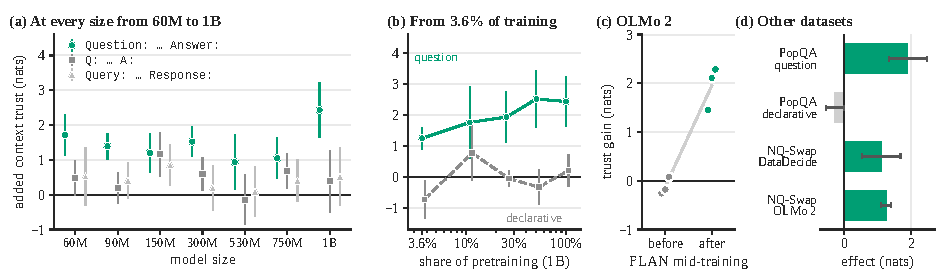
\includegraphics[width=\textwidth]{figures/fig4_question.pdf}
  \caption{\textbf{The \tmpl{Question:} habit across sizes, training and datasets.}
  Added trust in a counterfactual context (log-probability margin of the counterfactual over the memorized answer, relative to a declarative prompt; nats, $\pm$ SE).
  (a)~Flan minus no-Flan DataDecide models at every size, for the Flan template and two equivalent templates.
  (b)~During pretraining of the 1B models: present at the first checkpoint (3.6\%); declarative prompts unaffected.
  (c)~OLMo~2 1B before and after mid-training on a mixture with 16.6\% FLAN (three mid-training runs).
  (d)~PopQA counterfactuals and NQ-Swap (\tmpl{Question:} vs.\ \tmpl{Q:}).}
  \label{fig:question}
\end{figure*}
% generated by scripts/tables_acl.py -- do not edit by hand
\begin{table*}[t]
  \centering
  \footnotesize
  \setlength{\tabcolsep}{4.5pt}
  \begin{tabular}{@{}lcccccc@{}}
    \toprule
    Size & \tmpl{Question:}$q$\tmpl{Answer:} & \tmpl{Question:}$q$ & \tmpl{Answer:} & \tmpl{Q:}$q$\tmpl{A:} & \tmpl{Query:}$q$\tmpl{Resp.:} & other entity \\
    \midrule
    60M & +1.71 (0.58) & +0.73 (0.35) & +1.74 (0.59) & +0.48 (0.51) & +0.52 (0.83) & +2.14 (0.51) \\
    90M & +1.39 (0.37) & +1.23 (0.55) & +1.51 (0.17) & +0.20 (0.44) & +0.40 (0.52) & +1.89 (0.47) \\
    150M & +1.20 (0.57) & +1.09 (0.43) & +1.45 (0.70) & +1.16 (0.62) & +0.85 (0.59) & +1.48 (0.41) \\
    300M & +1.52 (0.44) & +1.60 (0.60) & +1.54 (0.50) & +0.58 (0.48) & +0.19 (0.65) & +1.37 (0.41) \\
    530M & +0.94 (0.79) & +0.96 (0.79) & +0.33 (0.70) & $-$0.14 (0.72) & +0.08 (0.72) & +1.51 (1.14) \\
    750M & +1.05 (0.59) & +1.72 (0.35) & +1.35 (1.40) & +0.68 (0.50) & +0.40 (0.61) & +2.17 (0.50) \\
    1B & +2.43 (0.79) & +2.04 (0.83) & +1.13 (0.63) & +0.39 (0.89) & +0.52 (0.83) & +3.06 (1.42) \\
    \bottomrule
  \end{tabular}
  \caption{\textbf{The \tmpl{Question:} habit at every size.} Flan minus no-Flan DataDecide models: added trust in the
  counterfactual context relative to a declarative ending, in nats (SE). Flan's template carries the effect at every
  size, and more than the equivalent \tmpl{Q:}/\tmpl{A:} and \tmpl{Query:}/\tmpl{Response:} templates at every size
  (pooled over sizes by $0.93 \pm 0.29$ and $0.98 \pm 0.32$ nats); below 1B, \tmpl{Answer:} alone often carries much
  of it.}
  \label{tab:habit_sizes}
\end{table*}

% generated by scripts/tables_acl.py -- do not edit by hand
\begin{table*}[t]
  \centering
  \footnotesize
  \begin{tabular}{@{}llrrr@{}}
    \toprule
    Model & Instruction data in pretraining & declarative & question & gain \\
    \midrule
    OLMo-1B (July 2024) & Dolma 1.7, with Flan & 4.33 & 8.92 & +4.60 \\
    Qwen2.5-1.5B & synthetic data from instruct models & $-$0.47 & 2.70 & +3.18 \\
    Pythia-1B & none (the Pile) & 5.47 & 6.89 & +1.41 \\
    Pythia-1.4B & none (the Pile) & 5.41 & 6.78 & +1.38 \\
    SmolLM2-1.7B & not documented & 2.89 & 3.93 & +1.04 \\
    Gemma-2-2B & not documented & 3.48 & 4.51 & +1.03 \\
    OLMo-2-1B, before mid-training & none & & & $-$0.26 to +0.08 \\
    OLMo-2-1B, after mid-training & 16.6\% FLAN & & & +1.45 to +2.28 \\
    \bottomrule
  \end{tabular}
  \caption{\textbf{The habit in public base models.} Trust in a one-sentence counterfactual context (nats) with a
  declarative ending and with a \tmpl{Question:}/\tmpl{Answer:} ending, and the gain from the question format.
  The model pretrained with Flan trusts a question most.}
  \label{tab:public}
\end{table*}

\paragraph{Prompts.} Context $S$ = the first sentence of a ParaConflict substitution conflict; declarative: $S$ + answer stem; QA: $S$ + \tmpl{Question:} $q$ \tmpl{Answer:} + stem; variants replace the markers (Table~\ref{tab:template}).
\paragraph{Items.} Facts known to every compared model (the memorized answer is more likely than the counterfactual without context): 1{,}680 ParaConflict items over six relations, 1{,}299 PopQA items, and 3{,}533 (DataDecide) and 3{,}750 (OLMo~2) NQ-Swap items. Standard errors use the seed-to-seed variance pooled over four 1B recipes with three seeds each.
\paragraph{Across sizes, training and datasets.} The habit is present at six of seven sizes from 60M to 1B (Figure~\ref{fig:question}a, Table~\ref{tab:habit_sizes}), appears by 3.6\% of pretraining and grows to $+2.4$ nats (Figure~\ref{fig:question}b), and replicates on PopQA counterfactuals ($+1.91$) and on NQ-Swap, where on natural reading-comprehension passages it is strongest after \tmpl{Question:} and extends to \tmpl{Q:} (Figure~\ref{fig:question}d).
In OLMo~2, mid-training on a mixture containing FLAN raises it from $\approx$ 0 to $+1.4$--$2.3$ nats in each of three runs, while trust under declarative prompts falls (Figure~\ref{fig:question}c); the mixture contains other data as well, so this replication shows the habit in a second training stack rather than isolating FLAN.
Continued pretraining of a Flan-free 60M model on 90M Flan tokens does not install it ($+0.04 \pm 0.04$).
\paragraph{Public models.} Table~\ref{tab:public} gives the trust of public base models with and without the question format.

\section{Artifacts, Compute and Software}
\label{app:artifacts}
\paragraph{Artifacts.} We use the DataDecide models (Apache~2.0) and data recipes (ODC-BY), Pythia and PolyPythias (Apache~2.0), OLMo~2 (Apache~2.0), ParaConflict (Apache~2.0), NQ-Swap (MIT) and PopQA as released by their authors, all for research use consistent with their intended use; the corpora are English.
\paragraph{Compute.} All experiments ran on NVIDIA A100 80GB GPUs, about 150 GPU-hours in total, including exploratory runs; most of it went to the controlled pretraining runs, while measuring the public checkpoints takes a few minutes per model.
\paragraph{Software.} PyTorch 2.8, Hugging Face Transformers 4.57 and Datasets 4.8, NumPy 1.26 and SciPy 1.17; models are loaded in bfloat16 with eager attention to read attention patterns. Benchmark scores are DataDecide's released OLMES evaluations \citep{magnusson2025datadecide}; marker counts in Dolma~1.7 come from the infini-gram index.

\section{Statistics}
\label{app:stats}
Recipe-bootstrap 95\% intervals for same- minus different-initialization agreement; unbiased two-way variance components from mean squares with $F$ tests; permutation tests with recipe labels permuted; Mantel tests for pair-level regressions \citep{mantel1967detection}; partial Spearman correlations by rank regression.

\end{document}
